%\documentclass[a4paper,12pt]{article}
\documentclass[letterpaper, 11pt, conference]{ieeeconf}
\usepackage{amsmath} % For 'cases' curly brace
\usepackage{amsfonts} % For bold number set font
\usepackage{graphicx}
\usepackage[font=bf]{caption}
\begin{document}
\title{\LARGE \bf
Mixed Non-Bayesian and DeGroot Learning
}
\author{Pedro d'Aquino\\pdaquino@umich.edu \and Dan Clark\\ddclark@umich.edu}
\date{December 11, 2012}

\maketitle

\begin{abstract}
We consider a model of social learning in which the network consists of two distinct types of agents: nodes following the Non-Bayesian update rule developed by Jadbabaie et. al. are interspersed with non-observant nodes performing simple DeGroot-style belief updates.  We develop a model that allows these types of update rules to coexist, and we consider implications on belief convergence.  We present simulations of our model for a variety of network structures and ratios of Non-Bayesian to DeGroot nodes.
\end{abstract}

\section{Introduction and Background}

Social learning is a process that occurs in a tremendous variety of settings; individuals and groups attempt to develop correct beliefs about complex issues such as economic patterns, social trends, and on new developments in technology.  Information may not always be easy to obtain in these situations.  Individuals receive a very limited picture of the true state of the world, and therefore must turn to neighbors in a social network to share opinions about these observations.  Thus we can think of the network as a whole attempting to learn the true state.

Many attempts have been made to model this phenomenon.  The DeGroot model of social influence proposes a system for reaching consensus where each node in a network adjusts their belief over time by linear combinations of their neighbors' beliefs~\cite{DeGroot1974}.  More sophisticated learning methods such as Bayesian inference provide algorithms for combining observations, neighboring opinions, and knowledge about network structure with prior beliefs to create a probability distribution over different belief states.  Jadbabaie et. al. propose a model for social learning that combines a Bayesian-style update with a simple linear inclusion of neighbors' opinions~\cite{Jadbabaie2012}.  They show that convergence to the correct belief about the state of the world is guaranteed under some straightforward assumptions about network connectivity and prior beliefs.

We seek to investigate the behavior of a network consisting of nodes learning in the ``Non-Bayesian'' style of Jadbabaie et. al. with the added presence of DeGroot-style nodes.  These DeGroot nodes will make no observations about the state of the world and incorporate neighboring beliefs in a simple linear manner.  This can model social learning scenarios where some members of a network thoughtfully develop beliefs based on observations and advice, and others do nothing but naively pass along opinions.  What are the consequences of such naive agents in a social learning scenario?  Do certain network structures exacerbate their impact?  How many naive agents can be present before learning becomes prohibitively difficult?  In this work we investigate answers to these questions and propose our model of mixed Non-Bayesian and DeGroot learning as a tool for future research.

\section{The Model}

\subsection{The Network}

The network in our model consists of an undirected graph where each vertex is either a Non-Bayesian or a DeGroot node.  At each discrete timestep $t$, every node will perform a belief update of its corresponding type.  If two vertices are connected by an edge, they are said to be neighbors and will incorporate each others' beliefs in their respective updates.

The model allows for a variety of generative methods to be used for creation of the network structure such as Erdos-Renyi, Watts-Strogatz, Kleinberg's Small-World Model, or a power law distribution.  We investigate several of these network types in simulation, described in section~\ref{sec:simulation}.

\subsection{States and Signals}

We will consider the state of the world to be a probability distribution $p^*(t) \in \mathbb{P}$.  $\mathbb{P}$ is a pre-defined class of distributions where each  $p^*(t) \in \mathbb{P}$ is distinguishable by a single parameter.  This single parameter $m^*$ where $\{m^* \in \mathbb{R}: m_{min} <= m^* <= m_{max} \}$  will be the state that the nodes in the network are attempting to learn.  That is, $m^*$ is the ``true'' state of the world.  \emph{A priori}, the nodes know the class of distribution but not the specific value of $m^*$; only that it lies uniformly in the range $[m_{min}, m_{max}]$.

Our model allows for $\mathbb{P}$ to be any class of probability distribution as long as it can be completely specified by a single parameter $m^*$.  Examples include the Poisson distribution with parameter $m^*$ and Gaussian distribution with mean $m^*$ and constant variance.  We also introduce a trapezoidal probability distribution in section~\ref{sec:trapezoidal_distribution} that serves as a valid choice for $\mathbb{P}$.

At each timestep $t$, every Non-Bayesian node $i$ will receive a signal $s_{i,t}$ that is a value drawn from $p^*(x)$.  These observations will be used by the nodes in the network to construct a belief about $m^*$.

\subsubsection{The Trapezoidal Distribution}
\label{sec:trapezoidal_distribution}

As an example of a class of distributions that can be used in our model we present the following trapezoidal distribution.

\begin{equation}
p^*(x)=\begin{cases}
m^* \cdot x + \frac{1}{2}(2-m^*) & 0 \le x \le 1 \\
0, & \text{otherwise}
\end{cases}
\end{equation}

The slope $\{ m^* \in \mathbb{R} : m_{min} = -2 \le m^* \le 2 = m_{max} \}$ will be the defining characteristic of the distribution.  We have chosen to bound $m^*$ between -2 and 2 and add the term $\frac{1}{2}(2-m^*)$ so that the support of $p^*(x)$  is always over $[0,1]$.

\begin{figure}[h]
\centering
%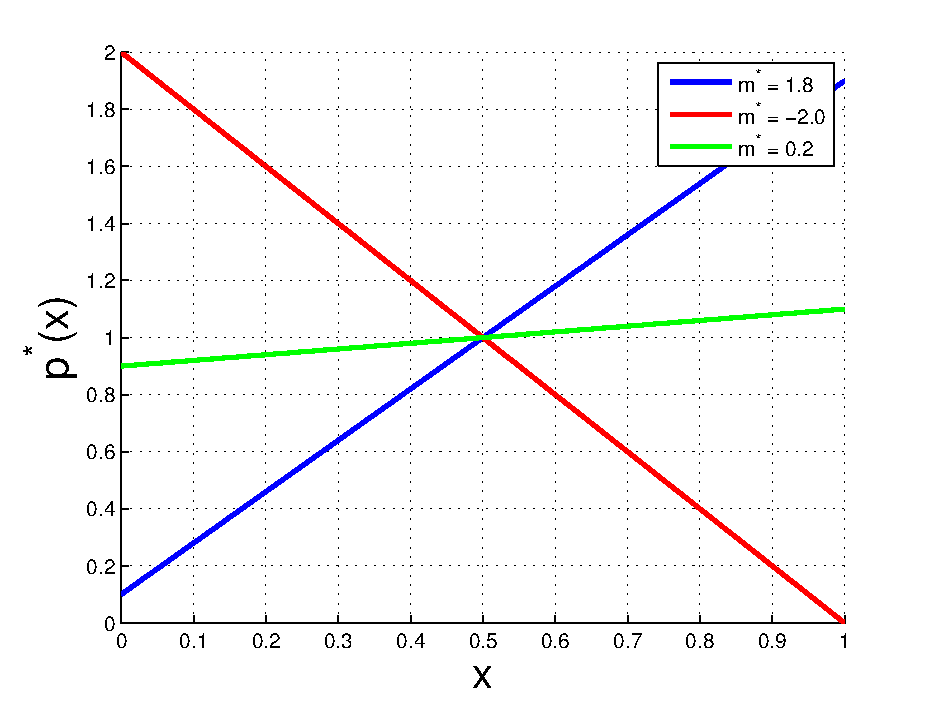
\includegraphics[scale=0.8]{trapezoidalDistribution}
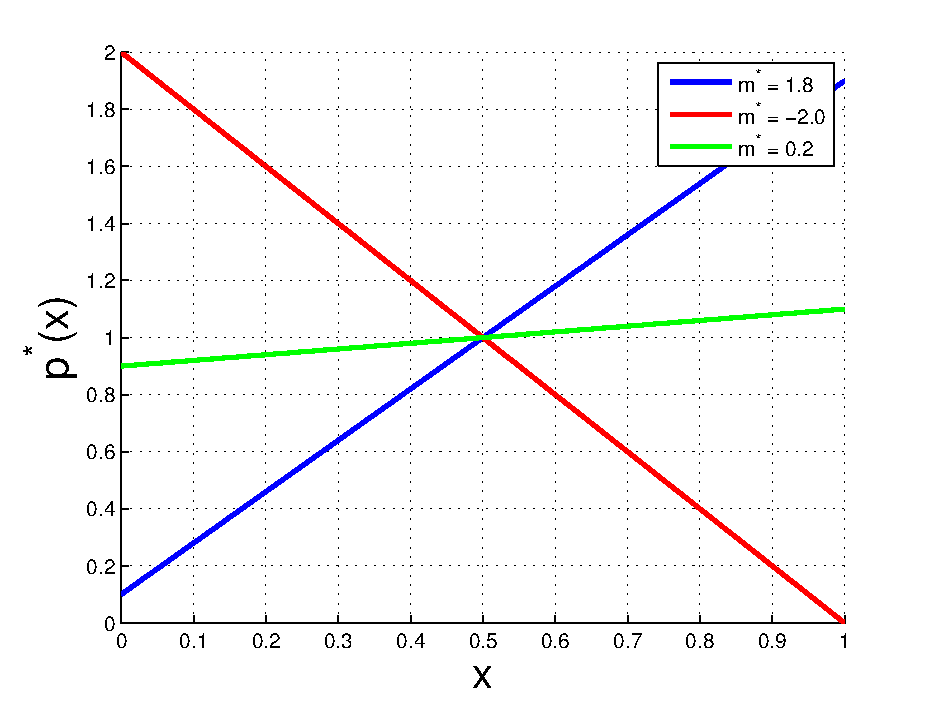
\includegraphics[width=0.48\textwidth]{trapezoidalDistribution}
\caption{Trapezoidal Probability Distribution}
\label{fig:trapezoidal}
\end{figure}

\subsection{Representing Belief States}

For a DeGroot node $i$, we represent the belief state of $i$ at time $t$ as a single value 
$m_{i,t} \in \mathbb{R}$.  However, belief of Non-Bayesian nodes is a probability distribution over a finite set of possible states of the world.  There is thus a tension between these two schemes and it is necessary to develop a conversion between the belief states of Non-Bayesian and DeGroot nodes.

\subsubsection{Belief in Non-Bayesian Nodes}

To represent a belief about the continuous slope value $m^*$ for a Non-Bayesian node we discretize $m$ in the following manner.  Let $\Theta = \{\theta_0, \theta_1,...\theta_n\}, n < \infty$ be the discrete set of possible states of the world over which each Non-Bayesian node holds a distribution of belief. Each $\theta_k$ corresponds to the belief that the slope of $p^*(x)$ is equal to $m_k$ where
\begin{equation}
\label{eq:theta_meaning}
\hat{m_k} = \frac{(m_{max} - m_{min})k}{n - 1} + m_{min}
\end{equation}
As an example, if we take $n = 21$ belief states, $m_{min} = -2$, and $m_{max} = 2$, then we have
\begin{equation}
\nonumber
\begin{cases}
& \theta_0: m^* = -2.0 \\
& \theta_1: m^* = -1.9 \\
& ... \\
& \theta_{20}: m^* = 2.0
\end{cases}
\end{equation}
For each Non-Bayesian node $i$, the belief at time $t$ that $\theta_k$ is the true state of the world is denoted by $\mu_{i,t}(\theta_k)$.  Thus $\{ \mu_{i,t}(\theta_1), \mu_{i,t}(\theta_2), ... \mu_{i,t}(\theta_n) \}$ is a probability distribution over the set of world states for fixed $i,t$.

\subsection{Learning in DeGroot Nodes}
DeGroot nodes in our model do not directly receive signals; they act merely as message-passers in the network.  For the most part our DeGroot nodes behave in a fashion similarly to nodes in a standard DeGroot-style network.  That is, a DeGroot node's $i$'s belief of the true slope value $m^*$ is given at time $t+1$ as
\begin{equation}
\label{eq:degroot_update}
m_{i,t+1} = \sum_{j \in N(i)} a_{ij}m_{j,t}
\end{equation}
where $N(i)$ denotes the neighbors of $i$.  $a_{ij}$ represents the level of ``trust'' that a DeGroot node $i$ has in neighbor $j$, such that

\begin{equation}
\nonumber
\sum_{j \in N(i)} a_{ij} = 1
\end{equation}
for all DeGroot nodes $i$.  Thus the DeGroot update in equation \ref{eq:degroot_update} is simply a weighted average of its neighbors' beliefs in the previous timestep.

When a DeGroot node with a Non-Bayesian neighbor performs an update it must obtain a value 
$m_{j,t}^\prime$ for the belief of this neighbor.  This is calculated as

\begin{equation}
m_{j,t}^\prime = \sum_{k=1}^n\mu_{j,t}(\theta_k)\hat{m_k}
\end{equation}

Here we are taking a weighted average of the $\hat{m_k}$ slope values represented by each state $\theta_k$ as defined in equation~\ref{eq:theta_meaning}, where the weights are given by $j$'s level of belief in each state.

\subsection{Learning in Non-Bayesian Nodes}

The update of a Non-Bayesian node in our model is handled similarly to the method laid out 
in \cite{Jadbabaie2012}.  We denote the belief of a node $i$ that it will receive the signal $s_i$ at time $t$ as $m_{i,t}(s_i)$, defined as follows:

\begin{equation}
m_{i,t}(s_i) = \int_\Theta \ell_i(s_i|\theta)d\mu_{i,t}(\theta) = \sum_{k=1}^n \ell_i(s_i|\theta_k)\mu_{i,t}(\theta_k)
\end{equation}

The likelihood function $\ell_i(s_i|\theta_k)$ can be obtained from the probability distribution function represented by the belief state $\theta_k$.  As an example, for the trapezoidal distribution described in section~\ref{sec:trapezoidal_distribution}, the likelihood function would be

\begin{equation}
\label{eq:likelihood}
\ell_i(s_i|\theta_k) \propto \hat{m_k} s_i + \frac{1}{2}(2 - \hat{m_k})
\end{equation}
where $\hat{m_k}$ is defined as in equation~\ref{eq:theta_meaning}.

The update of a node's belief in each state $\theta_k$ for a given time period $t$ is then given by

\begin{equation}
\label{eq:non_bayesian_update}
\mu_{i,t+1}(\theta_k) = a_{ii}\mu_{i,t}(\theta_k)\frac{\ell_i(\omega_{i,t+1}|\theta_k)}{m_{i,t}(\omega_{i,t+1})} + \sum_{j \in N(i)} a_{ij}\mu_{j,t}(\theta_k)
\end{equation}

Here the first term is the Bayesian update of the belief $\mu_{i,t}(\theta_k)$ after observing the signal $\omega_{i,t+1}$, multiplied by the node's self reliance $a_{ii}$.  The summation is the linear incorporation of the beliefs of $i$'s neighbors.

This update differs from the previous work in two major ways.  Firstly, we provide each Non-Bayesian node with only a single signal per timestep, where this signal is a single draw from the probability distribution $p^*(x)$.

Secondly, we must define $\mu_{j,t}(\theta_k)$ when $j$ is a DeGroot node.  We consider two methods for doing so, defined in sections \ref{sec:draw_from_degroot} and \ref{sec:likelihood_metric} respectively.

\subsubsection{Belief Distribution from Draw of Probability Distribution}
\label{sec:draw_from_degroot}

We require a method for converting a DeGroot node $j$'s belief $m_{j,t} \in \mathbb{R}$ to a series of priors that can be included in a Non-Bayesian node $i$'s belief update.  The first method we consider involves generating a probability distribution $p_{j,t}$ from $j$'s belief at time $t$ and drawing from this distribution.  The generated distribution is the $p_{j,t} \in \mathbb{P}$ where $j$'s belief $m_{j,t}$ is the single parameter defining the distribution.  If $\mathbb{P}$ is the trapezoidal distribution defined in section~\ref{sec:trapezoidal_distribution}, then for each DeGroot neighbor of $i$ at time $t$ we have

\begin{equation}
p_{j,t}(x)=\begin{cases}
m_{j,t} x + \frac{1}{2}(2-m_{j,t}) & 0 \le x \le 1 \\
0, & \text{otherwise}
\end{cases}
\end{equation}

This is simply the distribution that $j$ believes to be the state of the world.  We then draw a single signal $s_{j,t}^\prime$ from this distribution.  We create a belief distribution $\mu_{j,t}^\prime$ from $s_{j,t}^\prime$ by performing a Bayesian-style update with equal priors.

\begin{equation}
\mu_{j,t}^\prime(\theta_k) = \frac{\ell_i(s_{j,t}^\prime|\theta_k)}{\sum_{i=1}^{n} \ell_i(s_{j,t}^\prime|\theta_i)}
\end{equation}

This generated belief distribution $\mu_{j,t}^\prime$ is then used for the values of $\mu_{j,t}(\theta_k)$ for the DeGroot node $j$ in the Non-Bayesian update of equation~\ref{eq:non_bayesian_update}.

\subsubsection{Belief Distribution from Likelihood Distance Metric}
\label{sec:likelihood_metric}

The second method we consider for creating a probability distribution over the set of belief states $\Theta$ is to define a distance metric such that

\begin{equation}
\mu_{j,t}^\prime(\theta_k) \propto \frac{1}{(m_{j,t}-\hat{m_k})^2}
\end{equation}
where $\mu_{j,t}^\prime$ is the belief distribution that is used for the DeGroot node $j$'s values of $\mu_{j,t}(\theta_k)$ in the Non-Bayesian update of equation~\ref{eq:non_bayesian_update}.

Since $\mu_{j,t}^\prime$ must be a probability distribution we must normalize the values for each state with the value

\begin{equation}
q_{j,t} = \sum_{k=1}^n \frac{1}{(m_{j,t}-\hat{m_k})^2}
\end{equation}

Thus the calculation to create the DeGroot node's level of belief in each state $\theta_k$ is given by

\begin{equation}
\mu_{j,t}^\prime(\theta_k) = \frac{(m_{j,t}-\hat{m_i})^{-2}}{q_{j,t}}
\end{equation}

\begin{figure*}[t]
%\hspace*{0.1in}
%\centerline{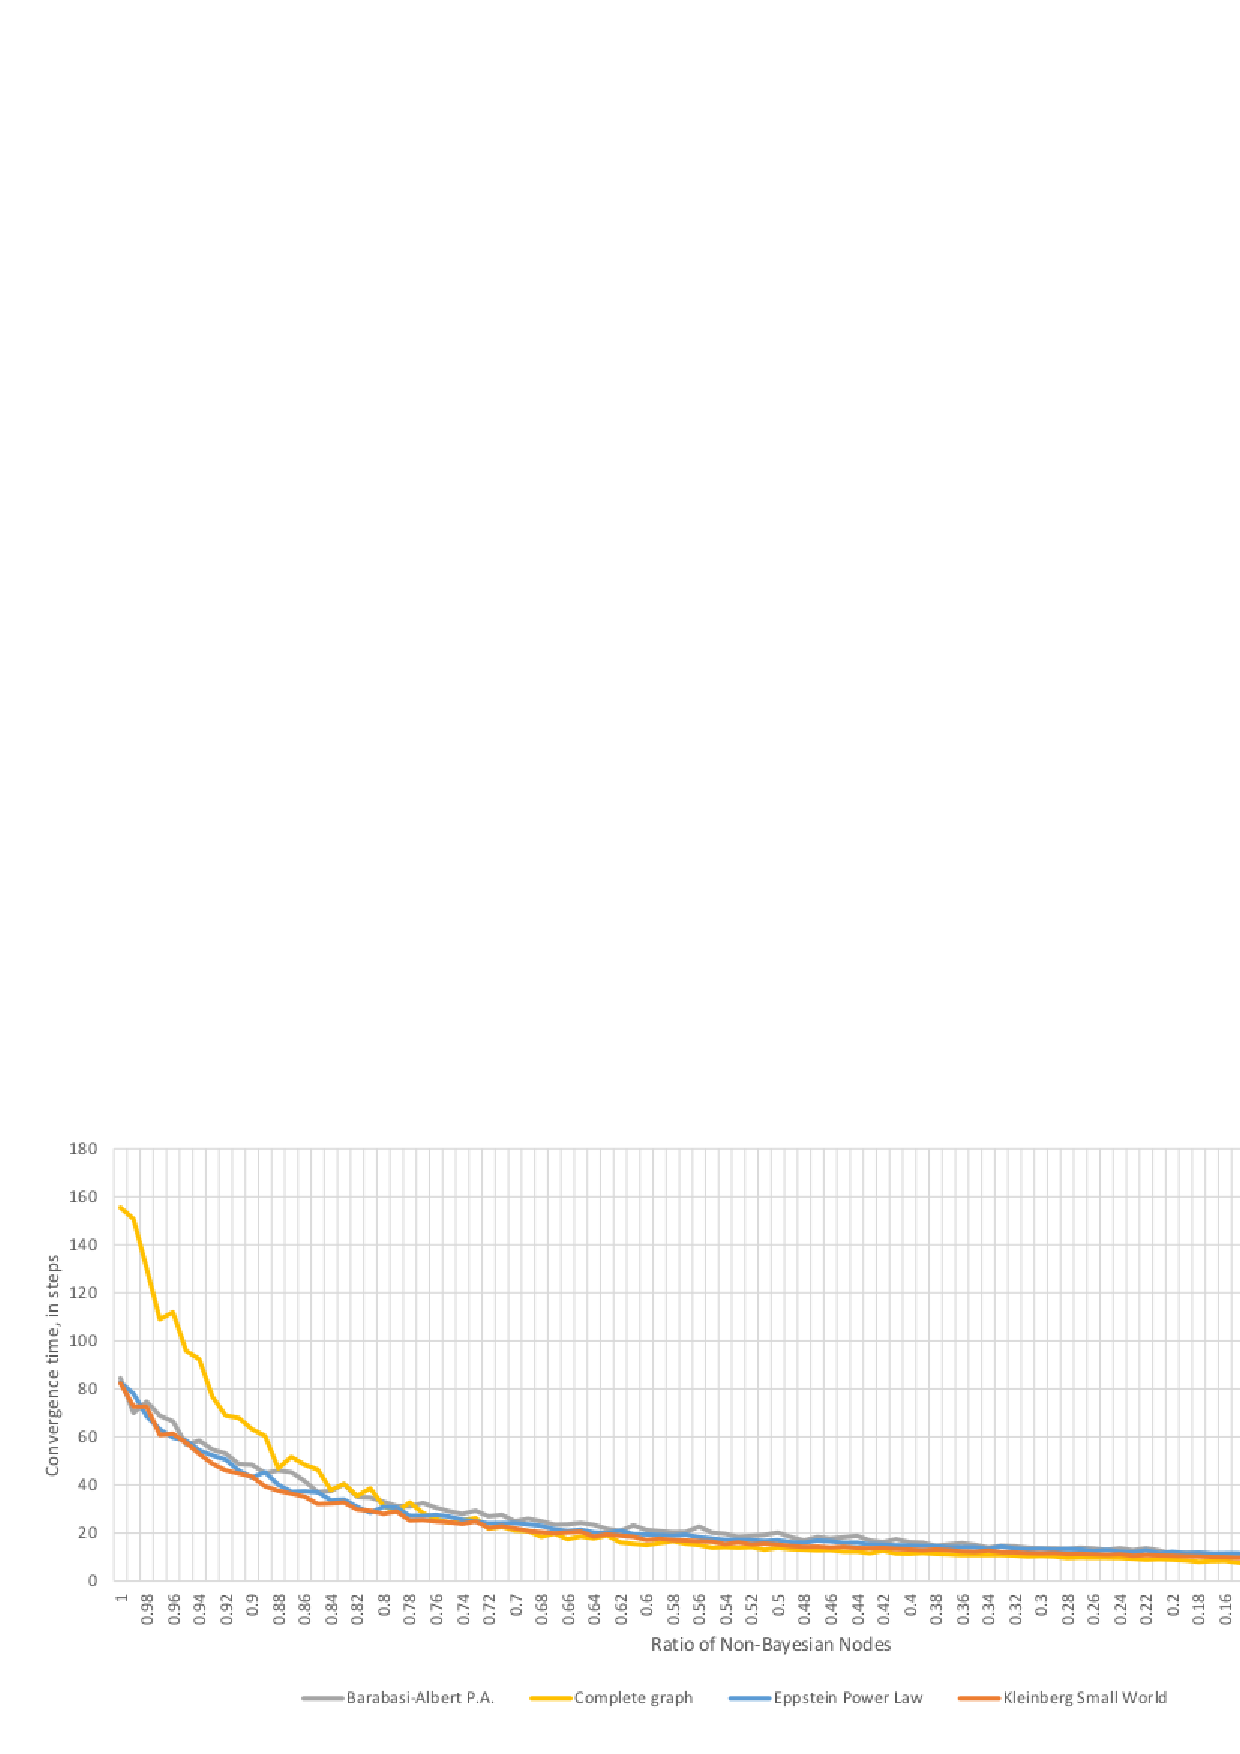
\includegraphics[scale=0.8]{figures/nb_ratio}}
\centering
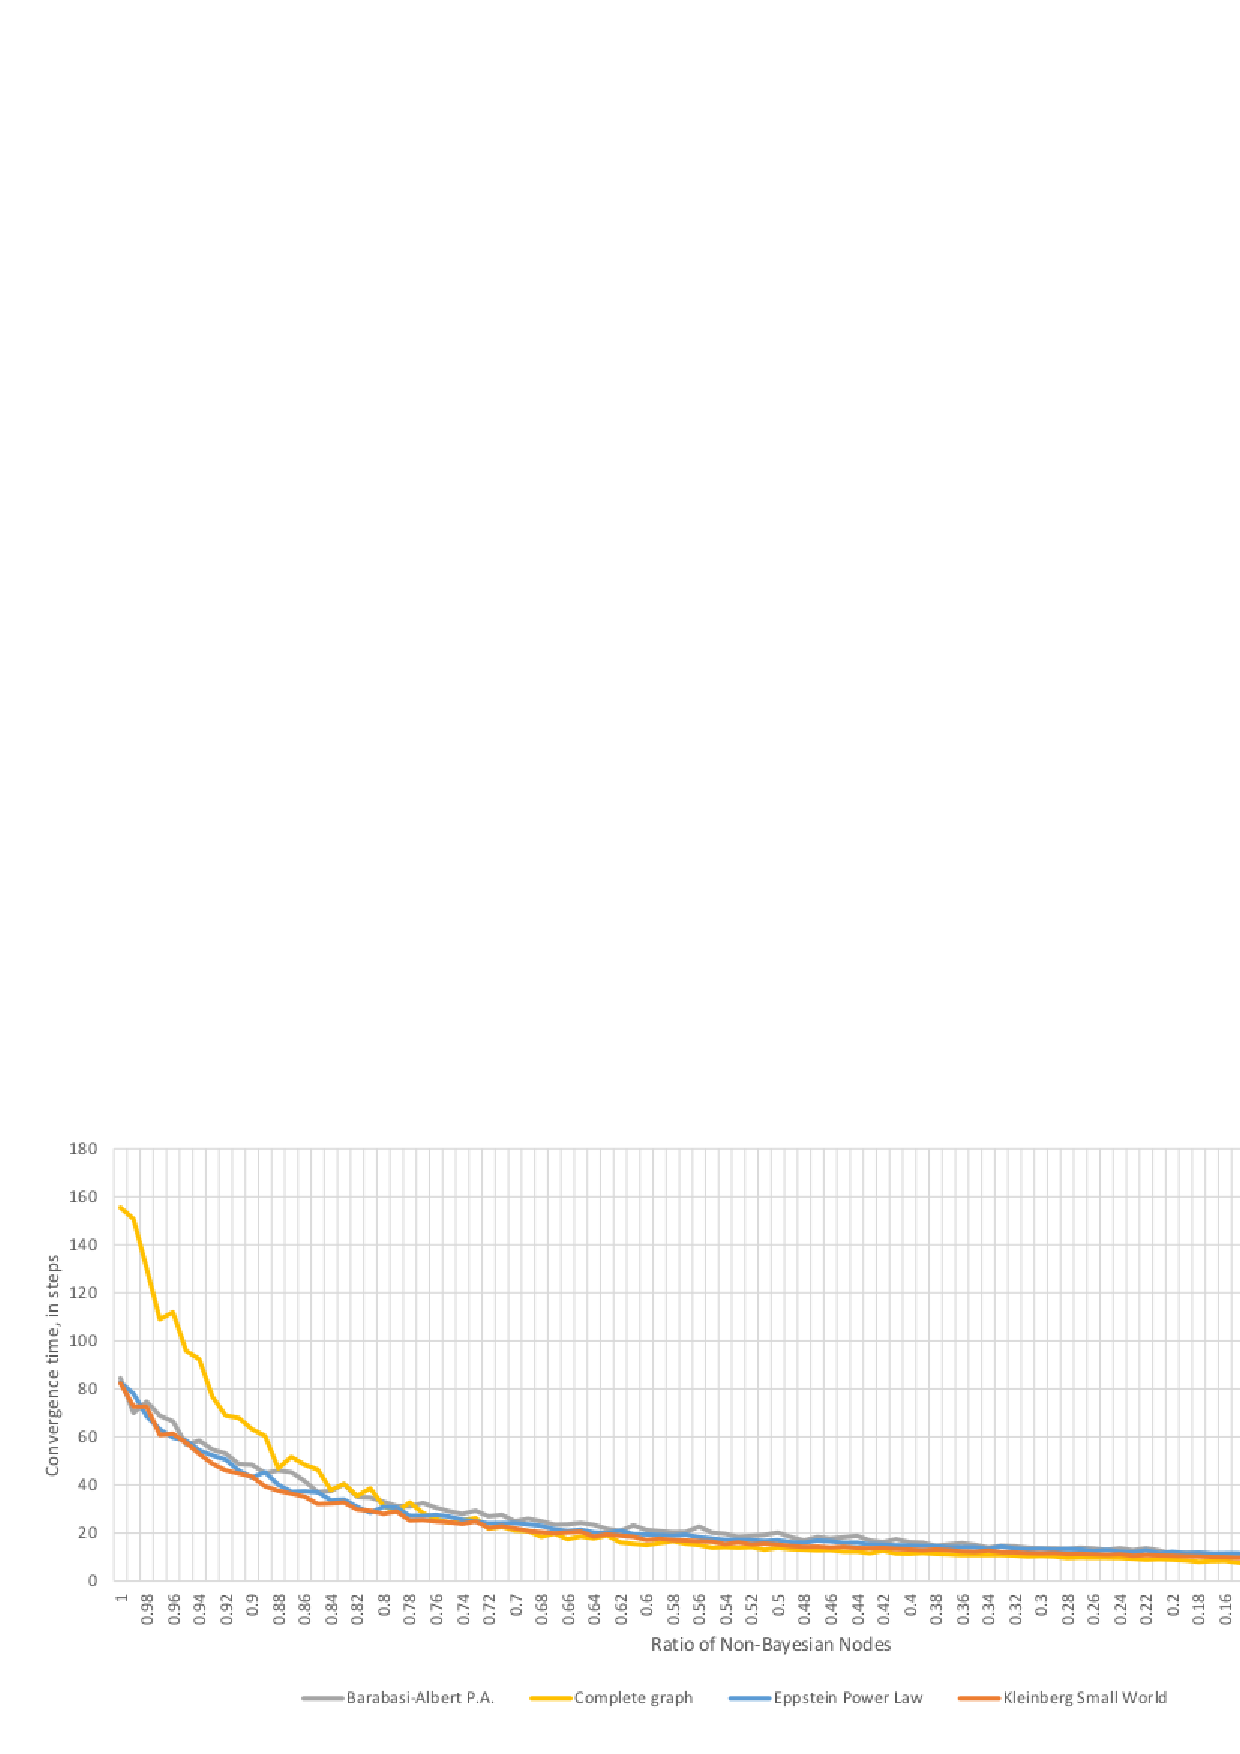
\includegraphics[width=0.9\textwidth]{figures/nb_ratio}
\caption{Time to convergence as the ratio of Non-Bayesian to DeGroot nodes decreases. For all trials the nodes had to distinguish between Gaussians centered at 100 and 105 with $\sigma=5$. To simulate the spread of information throughout the network, only 50\% of the Non-Bayesian nodes received any signals; the other 50\% needed to rely completely on learning from their neighbors. Each trial was run 100 times for each ratio percentage between from 1-100\%, for a total of 10,000 trials for each graph type. Unexpectedly, the time to convergence is inversely proportional to the ratio of Non-Bayesian nodes.}
\label{fig:nb_ratio}
\end{figure*}

\section{Convergence}
In this section we discuss theoretical results concerning convergence.  Here we define convergence as consisting of two parts: convergence for Non-Bayesian nodes and convergence for DeGroot nodes.  For a Non-Bayesian node $b$, we consider $b$ to have converged to a belief state $\theta_{k}$ if $\mu_{b,t}(\theta_k) \to 1$ as $t \to \infty$.  We consider a DeGroot node $d$ to have converged to the belief value $m$ if $m_{d,t} \to m$ as $t \to \infty$.  If these conditions hold for every Non-Bayesian and DeGroot node in the network, we consider the network to have converged.

We will demonstrate that convergence occurs for a very simple instance of our model, and then discuss difficulties encountered when attempting to extend these results.


\subsection{Convergence in a Simple Case}
Consider a network consisting of a Non-Bayesian node $b$ and a DeGroot node $d$ where $b$ and $d$ are connected and $d$ has a nonzero prior on the true state.  Suppose that $a_{dd}$ and $a_{bd}$ are strictly positive but that $a_{db} = 0$.  That is, the DeGroot node listens to the Non-Bayesian node but the Non-Bayesian does not consider the belief of the DeGroot node.

The update calculation for the Non-Bayesian node will then be 
\begin{equation}
\mu_{b,t+1}(\theta_k) = a_{bb}\mu_{b,t}(\theta_k)\frac{\ell_i(\omega_{b,t+1}|\theta_k)}{m_{b,t}(\omega_{b,t+1})}
\end{equation}

This is simply a Bayesian update based on $b$'s signal received at every timestep, so follows that $b$'s belief will converge to the correct value.  That is, $\mu_{b,t}(\theta^*) \to 1$ as $t \to \infty$ where $\theta^*$ is the correct belief state.


\begin{figure*}[t]
%\hspace*{0.1in}
%\centerline{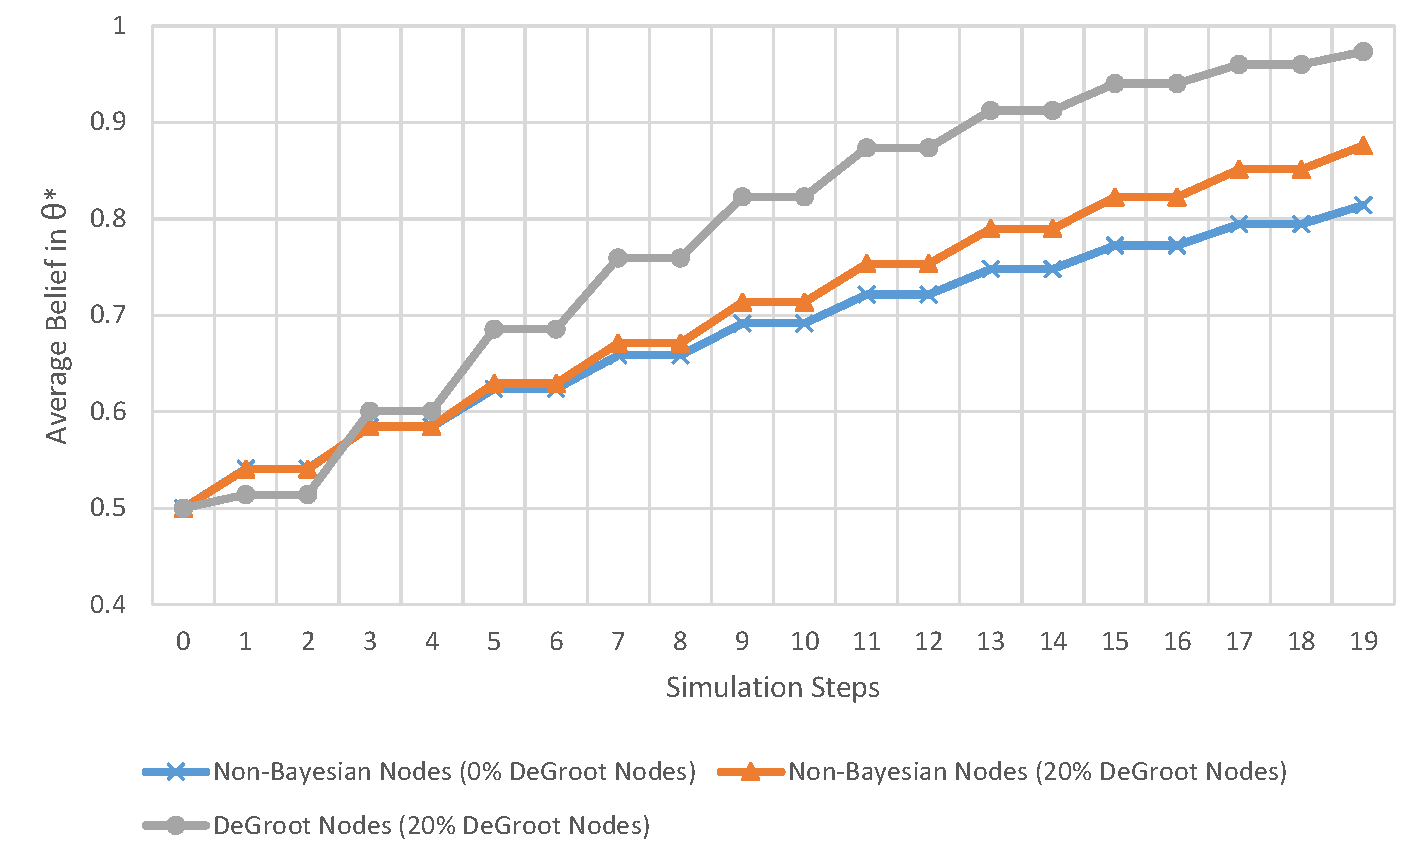
\includegraphics[scale=0.8]{figures/dg_faster}}
\centering
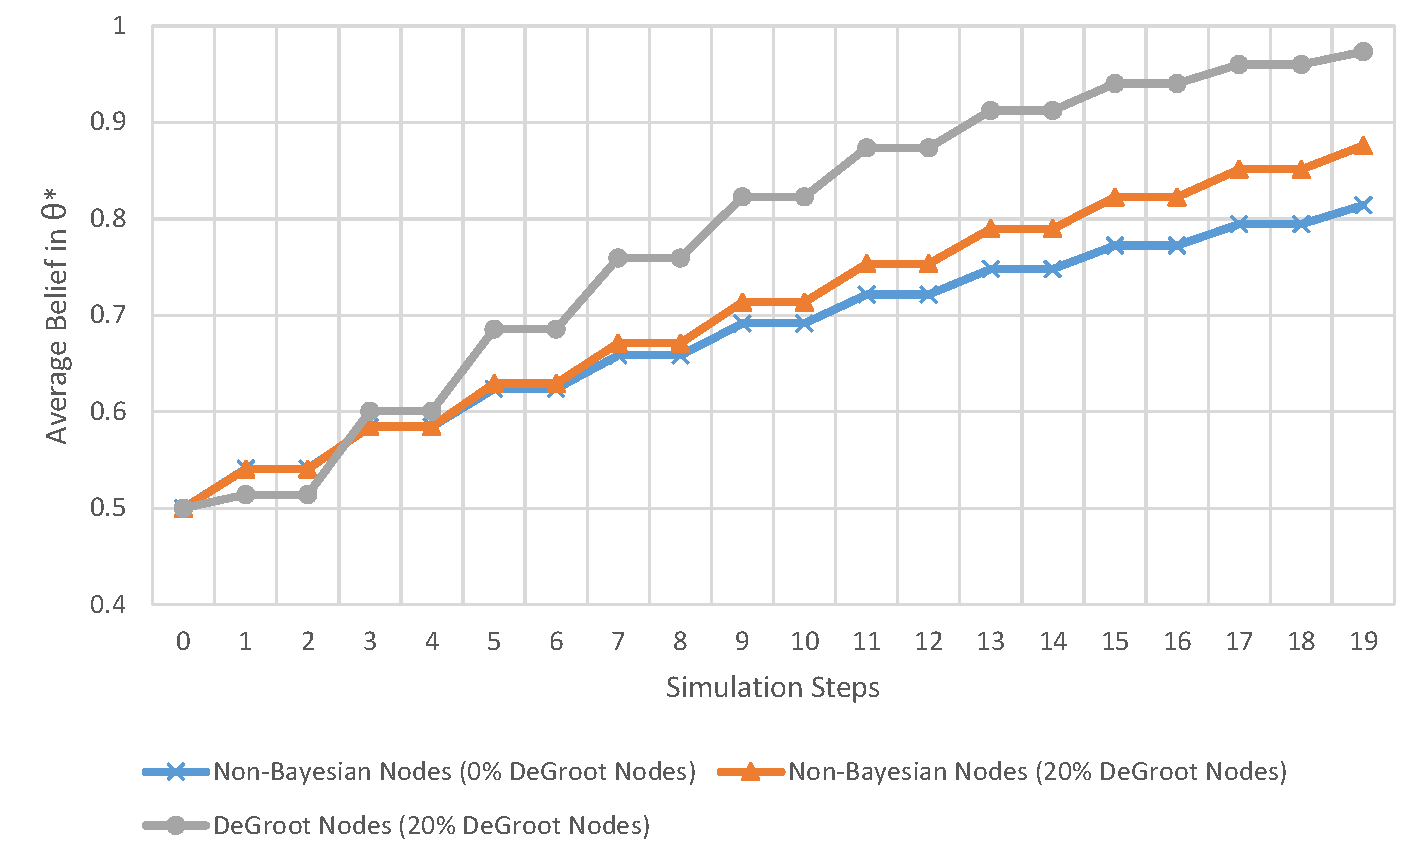
\includegraphics[width=0.9\textwidth]{figures/dg_faster}
\caption{The average beliefs in $\Theta^*$, the true distribution, for the two types of nodes during simulations with 0\% and 20\% of DeGroot nodes in a complete graph. The possible distributions were Gaussians centered at 100 and 105 with $\sigma=1$. All random seeds were fixed such that in both runs the Non-Bayesian nodes received the exact same sequence of draws. DeGroot nodes' beliefs were estimated using the distance metric. The figure shows how DeGroot nodes help amplify the initial belief updates of Non-Bayesian nodes, which leads to overall faster convergence.}
\label{fig:dg_faster}
\end{figure*}

The DeGroot node $d$'s update calculation will be
\begin{equation}
m_{d,t+1} = a_{db}\sum_{i=1}^n\mu_{d,t}(\theta_i)\hat{m_k}
\end{equation}

Once $b$ has converged to the correct state this will reduce to 

\begin{equation}
m_{d,t+1} = a_{db}\hat{m_{\theta^*}} = m^*
\end{equation}

Thus we observe that the network consisting of a DeGroot node listening to a Non-Bayesian node will converge to the correct belief.

\subsection{Difficulties in Extending Convergence Results}
Consider the simple network described in the previous section with the modification that $a_{bd}$ is strictly positive, so that the Non-Bayesian node takes into account the belief of the DeGroot node.  We then have

\begin{equation}
\mu_{b,t+1} = a_{bb}\mu_{b,t}(\theta_w)\frac{\ell_i(\omega_{b,t+1}|\theta_k)}{m_{b,t}(\omega_{b,t+1})} + a_{bd}\mu_{d,t}^\prime(\theta_w)
\end{equation}
where the term $\mu_{d,t}^\prime(\theta_w)$ depends on the method used to convert DeGroot to Non-Bayesian belief.  The methods we consider in sections \ref{sec:draw_from_degroot} and \ref{sec:likelihood_metric} both inject a level of noise into the network during each belief update through this term.

Noise from section~\ref{sec:draw_from_degroot}'s method results from the fact that we are performing a random draw from a probability distribution $p_{j,t}$ created from the parameter $m_{j,t}$ that may be different from the true value $m^*$.  Even if many draws are performs and averaged so that the ``signal-to-noise'' ratio is increased, the inclusion of data from a potentially incorrect probability distribution will still inject error into the network.

The likelihood metric method discussed in section~\ref{sec:likelihood_metric} also introduces error.  Even if the DeGroot node $d$'s belief $m_{d,t}$ has converged to the correct value $m^*$, we still have
\begin{equation}
\mu_{d,t}^\prime(\theta_w) \propto e^{-(m_{d,t} - \hat{m_w})^2} > 0
\end{equation}
for each incorrect state $\{ \theta_w \in \Theta : \theta_w \neq \theta^* \}$.  This will result in a small amount of noise added to each update of $d$'s neighbors' beliefs.

We have observed in simulation that the noise from the DeGroot to Non-Bayesian conversion can overcome the rate of learning from the signal observations and thus prevent convergence of the network.  However, it is difficult to determine exactly what conditions must hold for this to be the case.  The level of impact from the conversion noise will depend on many factors including network structure, trust values between nodes, and the number of states $\theta_i \in \Theta$ used to quantize possible values of $m^*$.  We have therefore found it difficult to prove convergence results with any significant level of generality.

\section{Simulation}
\label{sec:simulation}

\begin{figure*}[t]
%\hspace*{0.1in}
%\centerline{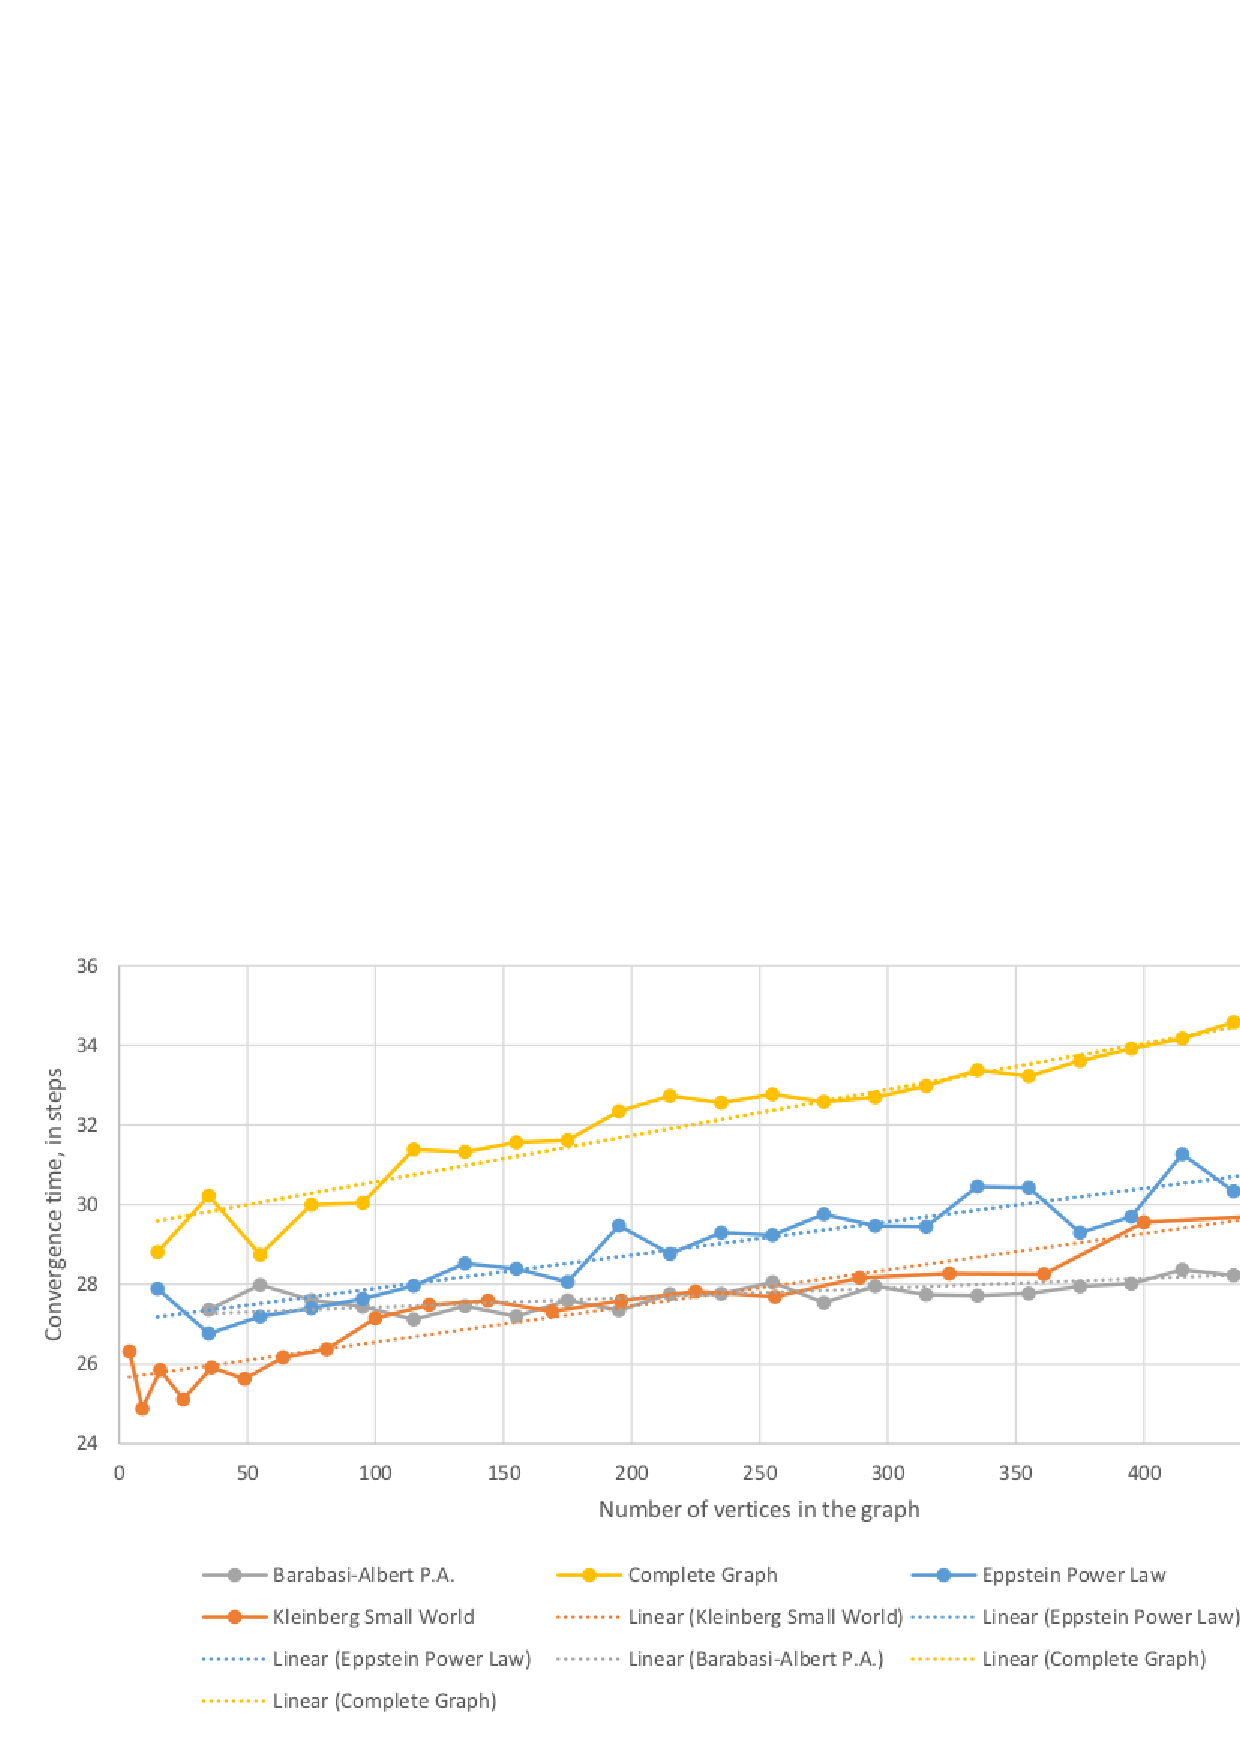
\includegraphics[scale=0.8]{figures/convergence_time}}
\centering
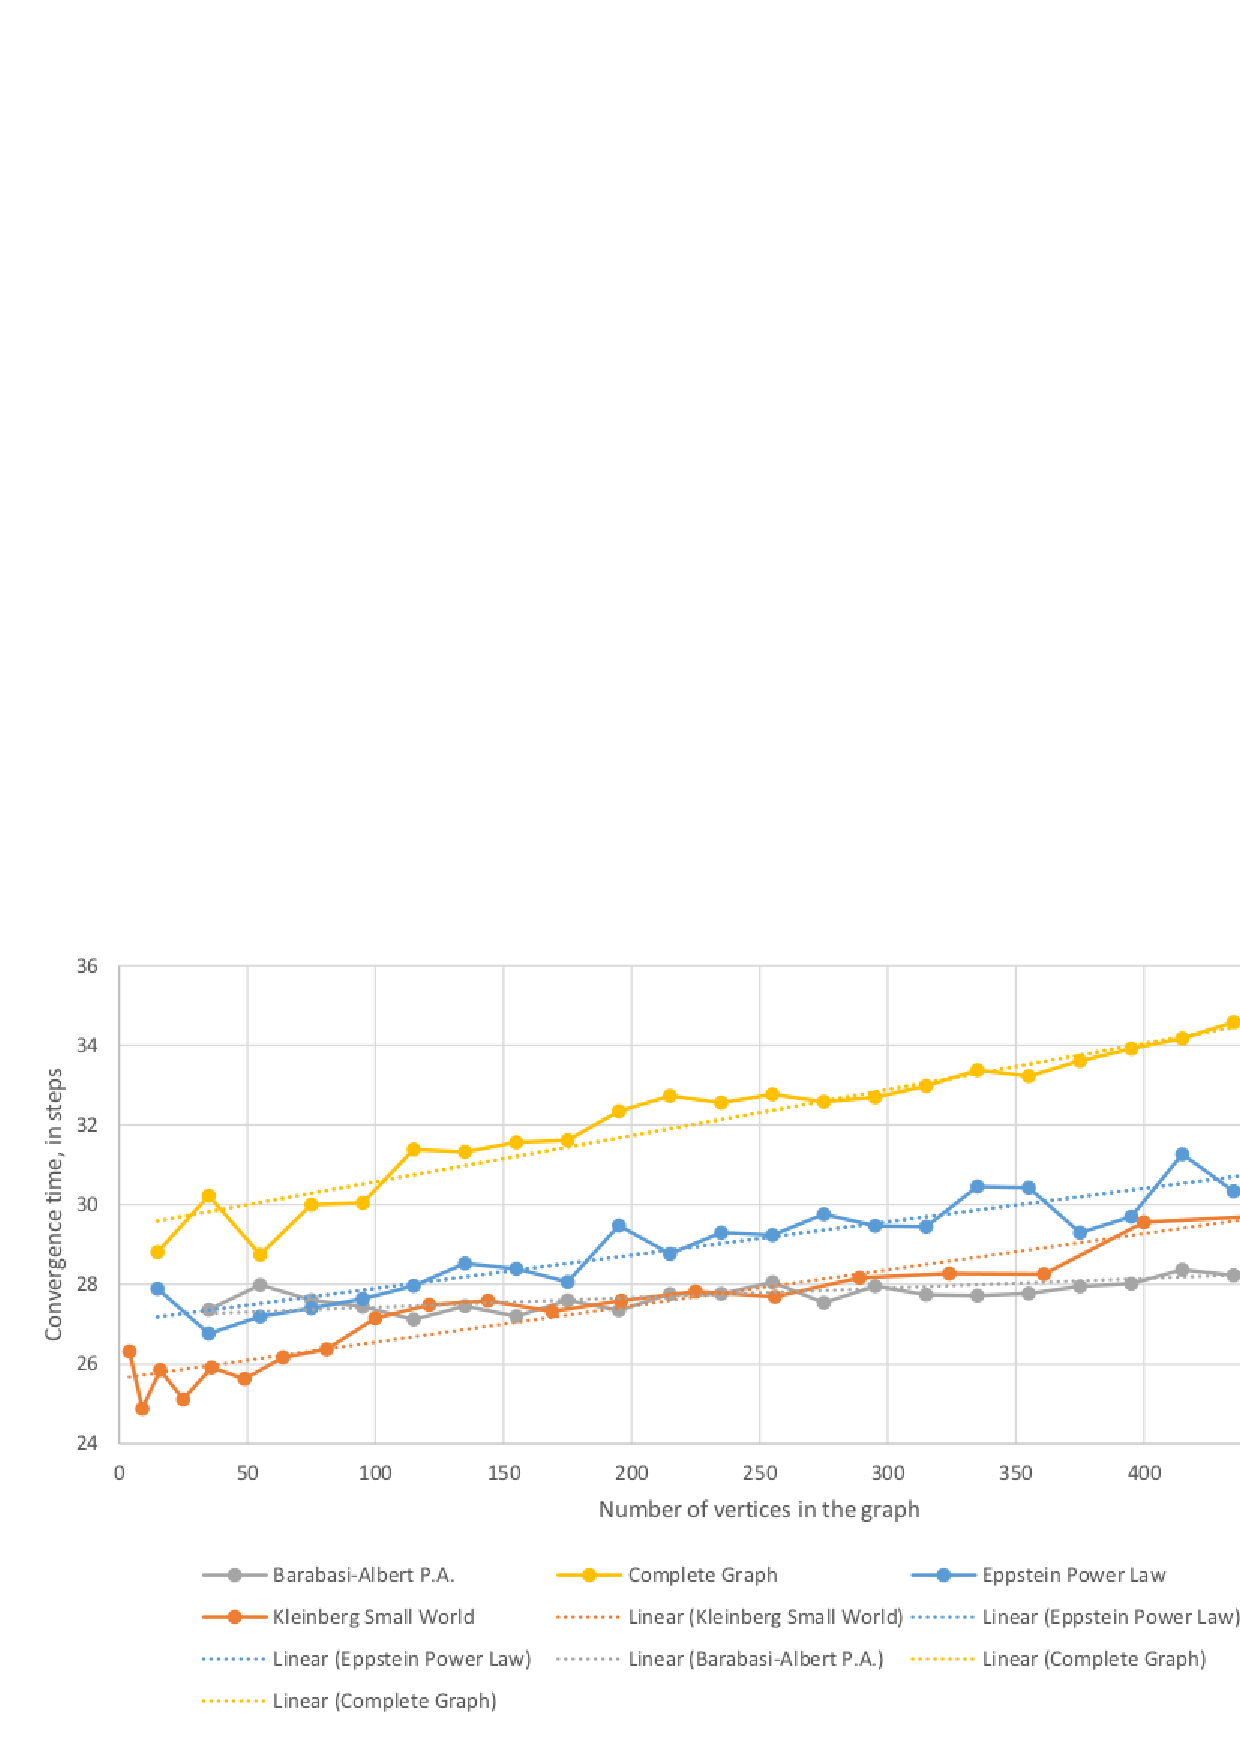
\includegraphics[width=.9\textwidth]{figures/convergence_time}
\caption{Time to convergence as the size of the graph grows. Each datapoint is the average of 200 trials. For all trials the nodes had to distinguish between Gaussians centered at 100 and 105 with $\sigma=5$. DeGroot nodes were on average 20\% of the total vertices. Only 60\% of the Non-Bayesian nodes were receiving signals. We also show $R^2$ values for a linear regression for the different types of graph. We can see that the convergence time increases linearly with the size of the graph, and that the complete graph takes substantially longer to converge. }
\label{fig:convergence_time}
\end{figure*}

In order to seek insight about the behavior of our model we performed a series of simulations using the JUNG network/graph software library \cite{website:JUNGGraphLibrary}.  For each simulation, $\Theta$ consisted of two Gaussian distributions with means of 100 and 105 and standard deviation of 1.  Each trial was run until all nodes have converged upon the true state or some maximum number of timesteps had elapsed.

\subsection{Random Draw Belief Conversion Method}

An important discovery from simulation was that the random draw method of conversion from DeGroot to Non-Bayesian belief described in section~\ref{sec:draw_from_degroot} can lead to unrealistically skewed belief distributions.  This primarily occurred in cases using Gaussian distributions where the means of the possible distributions represented by each belief state $\theta_i \in \Theta$ are relatively far apart.  For example, suppose that $n = 2$, $\theta_0 \sim N(100, 1)$ and $\theta_1 \sim N(105, 1)$.  A DeGroot node $d$ will have an initial belief of 102.5, and will therefore create a Bayesian belief distribution by drawing from the distribution $N(102.5, 1)$.  There is now a significant (0.318) probability that it will draw a point at least one standard deviation outside of the mean, e.g. $s_{d,t}^\prime = 101.5$.  But the value 101.5 is significantly more likely to have been drawn from the probability distribution $N(100, 1)$ versus the distribution $N(105, 1)$.  Therefore $d$ will report that it is almost certain that the true state is $\theta_0 \sim N(100, 1)$ when in reality it should have a relatively evenly spread belief distribution.

After the discovery of this difficulty, we evaluated the distance metric described in section~\ref{sec:likelihood_metric} and found it to give much more desirable results.  Therefore that method was used throughout all simulations described in the remainder of this section.

\subsection{Node Ratio vs. Convergence Time}
\label{sec:node_ratio_vs_convergence_time}

In order to characterize the effect of naive DeGroot nodes on Non-Bayesian social learning we simulated time taken for convergence versus the ratio of Non-Bayesian to DeGroot nodes in a network.  This simulation was performed for a several graph types: Barabasi-Albert preferential attachment~\cite{Barabasi}, Kleinberg small-world~\cite{KleinbergSmallWorld}, Eppstein power law~\cite{Eppstein}, and the complete graph.  


The results, shown in Figure~\ref{fig:nb_ratio}, are somewhat counterintuitive: the presence of naive DeGroot nodes actually tends to accelerate the speed of convergence.  Further investigation showed this to be a result of the process used to convert DeGroot beliefs to Non-Bayesian belief.  The conversion method of section~\ref{sec:likelihood_metric} tends to result in a belief distribution that is heavily skewed to a single $\theta_i$.  This relative ``certainty'' of the DeGroot nodes is picked up by their Non-Bayesian neighbors, bringing them more quickly to convergence.

We can see this process in more detail in Figure~\ref{fig:dg_faster}, which shows the average beliefs in $\Theta^*$ for the intial steps of two trials on a complete graph. It is clear that the DeGroot nodes essentially act as amplifiers, magnifying the initial belief updates of the Non-Bayesian nodes. This will in turn strengthen the Non-Bayesian's nodes beliefs in $\Theta^*$ (through Equation \ref{eq:non_bayesian_update}), which are then incorporated into the DeGroot nodes' parameter estimates. This feedback cycle increases the speed of convergence.

In essence, this happens because belief estimation algorithm of the DeGroot nodes is inherently aggressive. It is interesting to note that this can have negative effects on convergence when there is significant noise in the signal received by the Non-Bayesian nodes. If a Non-Bayesian node receives an ``unlucky'' draw that skews its belief distribution away from $\Theta^*$, this error will be amplified by the DeGroot nodes. Since there was no noise in our simulations, the presence of DeGroot nodes is beneficial. We find it interesting that the presence of naive, non-observant agents in a graph can actually accelerate the rate of learning due to eagerness of these nodes to settle on a single set of beliefs.


\subsection{Graph Size vs. Convergence Time}

We also evaluated time to convergence versus graph size for each of the network types tested in section~\ref{sec:node_ratio_vs_convergence_time}.  These simulations were performed with a ratio of 0.8 Non-Bayesian to DeGroot nodes, where 60\% of Non-Bayesian nodes received signals from the true probability distribution and 40\% had to rely completely on information from neighbors.

The results, shown in figure~\ref{fig:convergence_time}, show that time required for convergence appears to be linear with respect to the number of nodes in the graph.

\section{Conclusion}

We have developed a model that allows the Non-Bayesian social learning method of Jadbabaie et. al. to take place in a graph that also contains nodes performing simple DeGroot-style belief updates.  This model can be used as a theoretical framework for evaluating the effect that naive, non-observant agents can have on a network of more sophisticated learners.

We performed a series of simulations to obtain greater intuition about our model.  Some results were counterintuitive, such as the fact that DeGroot nodes can actually accelerate convergence due to a tendency towards certainty in their beliefs.

Future work could focus on proving further theoretical results for our model, such as specific conditions necessary to guarantee convergence.  This may involve development of different methods for converting DeGroot to Non-Bayesian belief that allow for easier theoretical analysis.  Future work could also investigate the effects of different choices for this method on convergence time.

\bibliographystyle{plain}
\bibliography{eecs598Report}

\end{document}
